In order to easily experiment with NUMA-aware task scheduling, we
implemented our own basic NUMA task scheduler. We call this scheduler
``Nas'' (NUMA Aware Scheduler) in the remainder of this paper. 

Nas design is similar to TBB, in that, tasks are objects containing an execute
method and some extra information such as dependencies.
We add NUMA node affinity into tasks objects to allow Nas scheduling
tasks with the best affinity. This NUMA affinity can be strict or not.
In strict mode, the tasks can only be executed on one NUMA node. In flexible
mode, tasks are executed in priority on the specified NUMA, but can also be
executed somewhere else if needed.

In Nas, threads of the same NUMA node share the same container of tasks, unlike
other runtimes that use one deque per thread. When a
task becomes available, it is put into the container corresponding to
its NUMA affinity if set,
otherwise a round robin algorithm is used by default. Because of thread concurrency
over the container, we didn't choose a simple deque but rather an optimized
structure which allows multiple operations at the same time.

Nas also provides control over data allocation and distribution
among NUMA banks, as well as memory block moves among NUMA banks.

Nas and Taggre are designed to cooperate together, with Taggre being
responsible for the DAG preprocessing, and Nas acting as the
runtime back-end. Both tools also cooperate together in controlling the placement of
tasks on the NUMA platform: The aggregation operator is called using
the Front algorithm with the number of NUMA nodes as parameter.

%-------------------------------
\subsection{NUMA helpers}
\label{NUMA_helper}
Nas has some NUMA helpers. The first helper is a function to allocate data
and distribute it over all NUMA banks. This is equivalent to starting a static
parallel for with OpenMP and First Touch policy activated, but in our case we have simplified this through a single function call. 
This helper is mainly useful for vector allocation.

The second helper is a function to move data between NUMA banks. The user registers the piece
of data and where he wants to move it. This helper is basically a wrapper for
the {\em move\_pages} system call. It automatically splits memory address and size into
a set of memory addresses aligned to page boundaries. This helper can be combined with Taggre
to distribute data by taking into account data access over computation time.
Thus, using Nas in conjunction with Taggre is a very convenient way to manage NUMA seamlessly in a task driven parallelization. 
Indeed, we provide a single function that uses the Taggre DAG to perform
an allocate or move memory pages of the data in order to balance the
work between sockets in accordance with the DAG. 
The task affinity with the sockets where its data are allocated is then
used by the scheduler to minimize the NUMA penalties. More details are
given in the next section.

%-------------------------------
\subsection{Nas with Taggre}
In order to optimize memory distribution, one can use the DAG of Taggre, and
Nas as runtime.
In most cases, tasks have data from other tasks to read in input and produce data
for other tasks in output. By distributing tasks over NUMA nodes, we can indirectly distribute
the data production. In most cases, the NUMA penalty of a write access is worst than
the NUMA penalty of a read access. The tasks distribution is done with the Front algorithm
and the number of NUMA nodes as parameter (Fig. \ref{fig:distrib_numa}).

Then we need to match the NUMA locality of data with the NUMA affinity of tasks which use it
by moving physical pages on the right NUMA bank.
To do this, we simulate an execution of the DAG with a user defined function. This
function is called for each task and must register data write in the
task to express that it should be brought them closer. 

In the case of GMRES, we distribute the row of the matrix following the DAG. All
vectors used during triangular solve are allocated using the first NUMA helper.


\begin{figure}[!t]
  \centering
  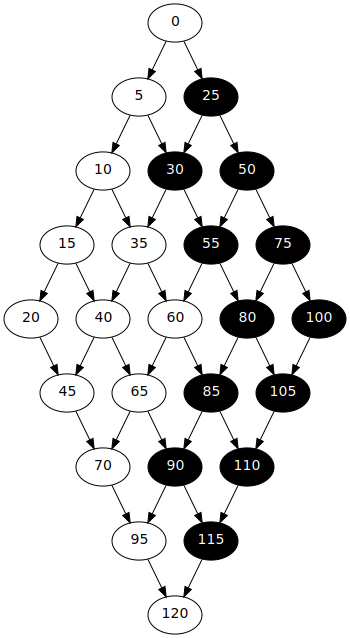
\includegraphics[width=2.5in]{numa_distrib}
  \caption{Distribution of tasks between 2 NUMA nodes, in white tasks of node 1, in black tasks of node 2}
  \label{fig:distrib_numa}
\end{figure}

%-------------------------------
\subsection{Result}
On a single 4-core socket, the Nas scheduler delivers results very similar to those
of TBB because no NUMA is involved. On our NUMA platform with two 4-core sockets,
the Nas scheduler delivers better results than TBB. On the
factorization step, we achieve an improvement
from 1 to 40\,\% (Tables~\ref{tab:full:8:facto:no},~\ref{tab:full:8:facto:nested}).

On the triangular solve step, the
improvement obtained with the Nas scheduler is 12.36\,\% on average
(Tables~\ref{tab:full:8:solve:no},~\ref{tab:full:8:solve:nested}). 
%% On Cube\_100 case, interleaved method is more effective than Nas method because of memory access
%% to the vector. For now, we allocate the vector with the first NUMA helper of Nas,
%% but during triangular solve, the first part of the vector is only write by first NUMA node, then
%% gradually the second NUMA node interleave some write in the middle part of the vector and finally only the second NUMA node
%% write the end of the vector. We are working on a generic way to optimize memory distribution.

On Cube\_100 case, one can notice that the interleaved memory allocation method
gives better results than using our NUMA aware allocator. This is due to the fact
that in the triangular solve, a task accesses the matrix data and some part of
the vector. The problem is that the matrix is allocated using the second NUMA helper
allocator (described in Subsection \ref{NUMA_helper}) whereas the vector is
allocated using the first NUMA helper allocator (optimized for the matrix-vector
product). Hence, the memory accesses to the vector are not optimized in the
triangular solve and the interleaved memory allocation method gives better results
in average. One can see that in the case SPE10 where each entry of the matrix
is a dense block (3,3), the memory accesses to the vector are more neglectable
and in this case the NUMA allocator is better.


%% \begin{table}[!h]
%%   \renewcommand{\arraystretch}{1.3}
%%   \caption{Results on the ILU(k) factorization step on two 4-core
%%     sockets with Nas with natural ordering}
%%   \label{tab:nas:8:facto:no}
%%   \centering
%%   \begin{tabular}{|c|c||c|c|}
%%     \hline
%%     Matrix & ILU & CD(4) & Improvement\\
%%     &     &  (speed-up) & compare to TBB\\
%%     \hline
%%     \hline
%%     & ILU(0) & 2.80 & 7.86\,\%\\
%%     CUBE\_100 & ILU(1) & 3.95 & 2.34\,\%\\
%%     & ILU(2) & 6.19 & 20.51\,\%\\
%%     \hline
%%     & ILU(0) & 5.34 & 39.77\,\%\\
%%     SPE10     & ILU(1) & 6.64 & 14.27\,\%\\
%%     & ILU(2) & 6.84 & 7.30\,\%\\
%%     \hline
%%   \end{tabular}
%% \end{table}
%% \begin{table}[!h]
%%   \renewcommand{\arraystretch}{1.3}
%%   \caption{Results on the ILU(k) factorization step on two 4-core
%%     sockets with Nas with nested dissection}
%%   \label{tab:nas:8:facto:nested}
%%   \centering
%%   \begin{tabular}{|c|c||c|c|}
%%     \hline
%%     Matrix & ILU & D(400) & Improvement\\
%%     &     &  (speed-up) & compare to TBB\\
%%     \hline
%%     \hline
%%     & ILU(0) & 3.95 & 17.56\,\%\\
%%     CUBE\_100 & ILU(1) & 5.14 & 2.24\,\%\\
%%     & ILU(2) & 5.72 & 1.00\,\%\\
%%     \hline
%%     & ILU(0) & 4.00 & 31.70\,\%\\
%%     SPE10     & ILU(1) & 5.57 & 8.72\,\%\\
%%     & ILU(2) & 6.06 & 6.49\,\%\\
%%     \hline
%%   \end{tabular}
%% \end{table}


%% \begin{table}[!h]
%%   \renewcommand{\arraystretch}{1.3}
%%   \caption{Results on the Triangular Solve step on two 4-core
%%     sockets with Nas with natural ordering}
%%   \label{tab:nas:8:solve:no}
%%   \centering
%%   \begin{tabular}{|c|c||c|c|}
%%     \hline
%%     Matrix & ILU & CD(4) & Improvement\\
%%     &     &  (speed-up) & compare to TBB\\
%%     \hline
%%     \hline
%%     & ILU(0) & 2.66 & 7.55\,\%\\
%%     CUBE\_100 & ILU(1) & 2.95 & 3.67\,\%\\
%%     & ILU(2) & 3.18 & 4.85\,\%\\
%%     \hline
%%     & ILU(0) & 3.24 & 26.68\,\%\\
%%     SPE10     & ILU(1) & 4.43 & 16.62\,\%\\
%%     & ILU(2) & 4.96 & 19.07\,\%\\
%%     \hline
%%   \end{tabular}
%% \end{table}

%% \begin{table}[!h]
%%   \renewcommand{\arraystretch}{1.3}
%%   \caption{Results on the Triangular Solve step on two 4-core
%%     sockets with Nas with nested dissection}
%%   \label{tab:nas:8:solve:nested}
%%   \centering
%%   \begin{tabular}{|c|c||c|c|}
%%     \hline
%%     Matrix & ILU & D(400) & Improvement\\
%%     &     &  (speed-up) & compare to TBB\\
%%     \hline
%%     \hline
%%     & ILU(0) & 1.92 & 14.49\,\%\\
%%     CUBE\_100 & ILU(1) & 2.07 & 7.02\,\%\\
%%     & ILU(2) & 2.24 & 6.73\,\%\\
%%     \hline
%%     & ILU(0) & 2.19 & 18.71\,\%\\
%%     SPE10     & ILU(1) & 3.08 & 12.49\,\%\\
%%     & ILU(2) & 3.32 & 13.42\,\%\\
%%     \hline
%%   \end{tabular}
%% \end{table}

